\chapter{Simulaciones Monte Carlo}


\newcommand{\mccaption}{La sección eficaz a LO para cada modo de decaimiento,
  los factores $k$ (para la normalización NLO) y las eficiencias del filtro
  están detalladas, así como también la luminosidad integrada correspondiente
  a la estadística total de cada muestra.}

%% \note{Mirar ``Perspective in SUSY II'' de Kane,
%% Capitulo 11}

\section{Generación de eventos de SUSY}

La conexión entre la teoría/fenomenología de SUSY (o cualquier otra teoría de
nueva física), y las observaciones experimentales en el detector de un
colisionador se realiza por medio de un \emph{generador de eventos}. Dada una
teoría de nueva física, que en general predice la existencia de nuevas
partículas y/o interacciones, el generador de eventos permite calcular cómo esa
teoría se manifiesta en el experimento.

El procedimiento, una vez que se selecciona un modelo particular de SUSY,
requiere de varios pasos que se encuentran esquematizados en la
\cref{fig:mc_sketch}.
En primer lugar es necesario calcular el espectro de masas de las partículas
supersimétricas, y sus acoplamientos. A partir de esto se calculan los anchos y
tazas de decaimiento de todas estas partículas. Y por último se utiliza el
generador, que toma como entrada las masas y decaimientos calculados previamente,
y genera los eventos de SUSY. Para los distintos pasos se utilizan
distintas herramientas por lo que es fundamental contar con un forma de poder
intercambiar información entre ellas de una forma estandarizada. Con este motivo
se creo un tipo de archivo llamado SLHA (SUSY Les Houches Accord)\cite{SLHA} que
puede funcionar como input/output de estas herramientas.

\begin{figure}[h]
  \centering
  \scalebox{0.8}{\begin{tikzpicture}[node distance=1.5cm, auto,]

    \node[rec] (susy) {\sc Modelo SUSY};
    \node[rec, right=of susy] (masses) {\sc Espectro de Masas};
    \node[rec, right=of masses] (decays) {\small \sc Decaimientos};
    \node[rec, right=of decays] (gen) {\sc Generador de Eventos};
    \node[rec, right=of gen] (atlas) {\sc Simulación Detector};

    \draw[arr] (1.7,0) -- (2.7,0);
    \draw[arr] (6.2,0) -- (7.2,0);
    \draw[arr] (10.8,0) -- (11.7,0);
    \draw[arr] (15.1,0) -- (16.1,0);

\end{tikzpicture}
}
  \caption{Etapas para la generacion de eventos de un modelo de SUSY.}
  \label{fig:mc_sketch}
\end{figure}



%% Para interfacear dos o mas calculos, el procedimiento general requiere que
%% el usuario prepare los parametros del modelo ,
%% junto con un conjunto de parametros
%% del SM (que seran usados como las
%% condiciones de contorno a escala de baja energia para el calculo del espectro),
%% en un archivo de texto , siguiendo el acuerdo SLHA.

%% Luego se corre un generador de espectro con este archivo como entrada para obtener
%% las masas de las particulas SUSY y los acoplamientos a la escala electrodebil.
%% El espectro resultante es guardado, junto con una copia de los parametros de entrada)
%% en un nuevo archivo.

%% El siguiente paso es utilizar un programa que genere los modos de decaimiento y sus anchos
%% para las particulas seleccionadas, que se guarda en un tercer archivo, junto con la copia
%% de los parametros de entrada y el espectro de masas.

%% Y por ultimo, se utiliza un generador de eventos (completo o a nivel partonico) que
%% genera los eventos a partir de la informacion de este archivo.


\subsection{Espectro de masas y decaimientos}

Los modelos de SUSY en lo que nos focalizamos suelen ser la teoria efectica a
bajas energias que resultan de una teoria mas general, como teoria de
supercuerdas, o que involucre un mecanismo particular para el rompimiento de
SUSY. Para especificar una teoria efectiva es necesario definir: (1) la simetria
de gauge, (2) los campos que la componen y, (3) el Lagrangiano. Los efectos del
rompimiento de SUSY estan codificados en los terminos de rompimiento soft del
Lagrangiano. Tambien se debe especificar la escala de energia a la cual la
teoria efectiva y el lagrangiano son validos. Y como los experimentos testean
fisica a la escala debil $Q\sim 1 \tev$, mientras que los parametros del
Lagrangiano son frecuentemente especificados a energias mucho mas altas
($M_\text{GUT}$ o $M_P$), debe usarse el grupo de ecuaciones de renormalizacion
(RGE) para conectars las dos escalas del modelo.

Una vez que los parametros del Lagrangiano son conocidos a la escala
electrodebil, pueden identificarse las masas fisicas de las particulas,
diagonalizando las matrices de masa correspondientes, y luego, para tener la
precision suficiente, aplicar las correciones a ordenes mayores (en general a 1
loop).

A partir del modelo también es posible calcular los anchos y tazas de decaimiento de todas las
partículas supersimetricas

Existen varios programas que permiten realizar estos calculos del espectro de
masas: \texttt{Isasugra}, \suspect, \texttt{SoftSusy} y \texttt{Spheno}...

En este trabajo utilizamos el programa {\susyhit}\note{ref} que combina
{\suspect} junto {\sdecay} y {\hdecay} para calcular los BRs y anchos de
decaimiento. Algunos de estos modos de decaimientos son calculados a NLO en QCD.



%% {\suspect}\note{referencia} corre las RGE a dos loops en el MSSM para determinar
%% los parametros de SUSY a la escala electrodebil en modelos de mSUGRA, GMSB, AMSB
%% y pMSSM. Y aplica luego las correscciones a 1 loop, y algunas correcciones a 2 loops
%% para las masas de los Higgs.



\vsp

Una vez que el espectro de masas y los decaimientos están calculados estos
pueden usarse como entrada en los generadores de eventos.

%% % SLHA
%% Para facilitar el intercambio de información entre distintos programas de SUSY
%% se propuso una seria de convenciones: SUSY Les Houches Accord (SLHA)\cite{SLHA}.
%% Este acuerdo permite usar la salida de los códigos que calculan el espectro de
%% masa y decaimientos como entrada en los generadores de eventos de una forma
%% consistente y sin ambigüedades.

%% %% En general estos modelos pueden
%% %% ser teorias efectivas
%% La teoria efectiva queda especificada adoptando la simetria de
%% gauge, the (super)field content y el Lagrangiano.
%% {\suspect} runs the 2-loop MSSM RGEs to determine weak scale
%% SUSY parameters in the mSUGRA, GMSB and AMSB models,
%% and in the pMSSM (a more general MSSM model). One-loop
%% sparticle mass corrections are included.
%% Some two loop corrections to Higgs masses are included.


\subsection{Generador de eventos}

Los programas descriptos anteriormente permiten pasar de un modelo de SUSY a las
predicciones en la producción de spartículas y sus anchos de decaimientos en
estados finales de quarks, leptones, fotones y gluones (y LSP en modelos donde
se conserva paridad-R). Sin embargo los quarks y gluones no pueden medirse
directamente en los detectores. Los detectores pueden medir trazas de partículas
(cuasi)estables cargadas y su momento en campos magnéticos, como también los
depósitos de energía en los calorímetros. Por lo tanto todavía falta un paso
entre estos modelos y las señales detectadas en los detectores, del cual se
encarga el generador de eventos. A partir de la colision hadronica inicial,
estos programas modelan la produccion de las particulas en el estado final a ser
medidas en el detector.

Para un dado tipo de colisionador y una dada energía de centro de masa, y un
modelo, el generador de eventos va a generar un conjunto eventos de pares de
spartículas de acuerdo a su sección eficaz. Estas partículas van a decaer
(posiblemente en en una cascada de varios pasos) en un estado final partónico,
de acuerdo a los BR fijados por el modelo. Este estado final partónico es
convertido en uno con partículas que puede ser detectadas en el detector.
Generando un gran numero de eventos de SUSY, se puede simular los posibles
estados finales que se esperada que un cierto modelo produzca.

%%Existen varios generadores que incorporan SUSY: \texttt{Isajet}, {\pythia}, {\herwig}, {\sherpa}.

La simulación de eventos de dispersión en colisionadores hadronicos puede
descomponerse en varios pasos descriptos a continuacion (y esquematizados en la
\cref{fig:mc_event_generator}):

\begin{itemize}

\item Interacción dura (HS):

  En este proceso, las particulas (en este caso protones) interactuan para
  producir las particulas fundamentales salientes primarias. Esta intraccion
  involucra los partones de los hadrones intervinientes en el proceso. El
  calculo se realiza, en general, a primer orden (LO) en teoria de perturbaciones,
  aunque algunos programas pueden incluir algunos procesos a NLO.
  Esta etapa tambien involucra la convolucion con las funciones de distribucion
  partonica (PDFs),

  %% El calculo perturbativo del proceso de interacción dura en el modelo
  %% partónico, y la convolución con las funciones de distribución partónica
  %% (PDFs),

\item Decaimientos:

  Las particulas suerpsimetricas producidas en la interaccion dura decaen (en general
  en forma de cascada) a otras particulas.

  %% la inclusión de los decaimientos en cascada de las sparticulas

  %% Las particulas fundamentales masivas, como el quark top,
  %%   los bosones de gauge electrodebiles, los bosones de Higgs y particulas de nueva fisica, decaen
  %%   en una escala de tiempo que es mas corta o comparable a las lluvias partinicas QCD.
  %%   Dependiendo de la naturaleza de las particulas y de si se producen particlas que interacctuen
  %%   fuertementen en el decaimiento, estas marticulas pueden tambien iniciar lluvias partonicas
  %%   antes y despues de su decaimiento.

\item Lluvias partonicas:

  Se implementa las lluvias partonicas, para las particulas producidas
  en la colision (lluvia de estado final o FSR), para los partones iniciales
  involucrados en la colision (lluvia de estado inicial o ISR), y tambien para otras
  particulas de color que puedan ser producidas como decaimiento de particulas mas pesadas.

  %% implementación de las lluvias de partones para los estados de partículas
  %% con color inicial y final, y para otras partículas con color que puedan ser
  %% producidas como decaimiento de otros objetos mas pesados,

\item Hadronización:

  En esta etapa se implementa el modelo de hadronización que describe la formación de
  mesones y bariones a partir de los quarks y gluones. También las partículas
  inestables deben decaer a partículas (cuasi) estables que son detectadas en el
  detector, con tasas y distribuciones que estén de acuerdo con los valores
  medidos o predichos.

\item Remanentes:

  Finalmente, los remanentes de los haces iniciales tienen que ser
  modelados para obtener una descripción valida de la física en las regiones
  forward del detector, lo que suele llamarse evento subyacente (UE).

\end{itemize}

\begin{figure}[h]
  \centering
  \includegraphics[width=0.6\textwidth]{figures/mc_event_generator}
  \caption{Distintas etapas implementadas en los generadores de eventos Monte Carlo.
    (1) Interaccion dura (HS), (2) Lluvias de estado inicial y final (ISR, FSR),
    (3) Decaimientos en cascada, (4) Hadronización, (5) Remanentes.}
  \label{fig:mc_event_generator}
\end{figure}




%% \note{del manual de Herwig}
%% Los procesos involucrados pueden dividirse en un numero de etapas
%% correspondientes al aumento de las escalas de  tiempo y distancia
%% involucradas:

%% \begin{enumerate}



%% \item Lluvias de partones de estado inicial y final:
%%     Las particulas de color en el evento son perturvativamente evolucionadas desde
%%     la escala dura de la colision hasta el corte infrarojo.
%%     Esto ocurre para las particulas producidas en la colision, la \emph{lluvia de estado final},
%%     y los partones iniciales involucrados en la colision, la \emph{lluvia de estado inicial}.
%%     La coherencia de la emision de gluones soft en las lluvias de partones de las particulas en
%%     la colision dura es controlada por el flujo de color de la colision dura.

%%     %% 3. Decay of heavy objects. Massive fundamental particles such as the top quark, electroweak
%%     %% gauge bosons, Higgs bosons, and particles in many models of physics beyond the Standard
%%     %% Model, decay on time-scales that are either shorter than, or comparable to that of the QCD
%%     %% parton shower. Depending on the nature of the particles and whether or not strongly interacting
%%     %% particles are produced in the decay, these particles may also initiate parton showers
%%     %% both before and after their decay. One of the major features of the Herwig++ shower
%%     %% algorithm is the treatment of radiation from such heavy objects in both their production
%%     %% and decay. Spin correlations between the production and decay of such particles are also
%%     %% correctly treated.
%%   \item Decaimiento de objetos pesados: Las particulas fundamentales masivas, como el quark top,
%%     los bosones de gauge electrodebiles, los bosones de Higgs y particulas de nueva fisica, decaen
%%     en una escala de tiempo que es mas corta o comparable a las lluvias partinicas QCD.
%%     Dependiendo de la naturaleza de las particulas y de si se producen particlas que interacctuen
%%     fuertementen en el decaimiento, estas marticulas pueden tambien iniciar lluvias partonicas
%%     antes y despues de su decaimiento.

%%   \item

%%     4. Multiple scattering. For large centre-of-mass energies the parton densities are probed in a
%%     kinematic regime where the probability of having multiple partonic scatterings in the same
%%     hadronic collision becomes significant. For these energies, multiple scattering is the dominant
%%     component of the underlying event that accompanies the main hard scattering. These
%%     additional scatterings take place in the perturbative regime, above the infrared cut-off, and
%%     therefore give rise to additional parton showers. We use an eikonal multiple scattering
%%     model [8], which is based on the same physics as the FORTRAN JIMMY package [18], together
%%     with some minor improvements. In addition to that we included non-perturbative
%%     partonic scatters below the infrared cut-off [19], which enables us to simulate minimum
%%     bias events as well as the underlying event in hard scattering processes.

%%     5. Hadronization.
%%     After the parton showers have evolved all partons involved in hard scatterings,
%%     additional scatters and partonic decays down to low scales, the final state typically
%%     consists of coloured partons that are close in momentum space to partons with which they
%%     share a colour index, their colour ‘partner’ (in the large Nc limit this assignment is unique).
%%     Herwig++ uses the cluster hadronization model [2] to project these colour–anticolour pairs
%%     onto singlet states called clusters, which decay to hadrons and hadron resonances. The
%%     original model of Ref. [2], which described this decay as pure phase space has been progressively
%%     refined as described in Sect. 7. Clusters that are too massive or too light for decay
%%     directly to hadrons to provide a good description are treated differently, again described in
%%     Sect. 7.

%%     6. Hadron decays. The hadron decays in Herwig++ are simulated using a matrix element
%%     description of the distributions of the decay products, together with spin correlations between
%%     the different decays, wherever possible. The treatment of spin correlations is fully
%%     integrated with that used in perturbative production and decay processes so that correlations
%%     between the production and decay of particles like the tau lepton, which can be
%%     produced perturbatively but decays hadronically, can be treated consistently.


%% \end{enumerate}

%% \subsubsection{Interacccion dura}

%% La interaccion dura y la convolucion con las PDFs es el calculo central
%% de los generadores de eventos. Los calculos se realizan generalmente
%% al orden mas bajo en teoria de perturbaciones, por lo que la interaccion
%% dura es un proceso de dispersion $2\to 2$ o $1\to 1$.


%% Finalmente, en un colisionador de hadrones, los remanentes del nucleon
%% que no participaron en la interaccion dura deben ser tenidos en cuenta.
%% Los efectos de los remanentes del haz producen un flujo de energia adicional,
%% especialemente en las regiones fast forward del detector. Existen distintas
%% formas de describir estos procesos no perturbativos. Adicionalmente, estos
%% remanentes deben ser hadronizados.


\subsection{Sección eficaz}

En el caso de procesos de producción de pares de gluino o quarks, de los cuales
existe el calculo a NLL, la sección eficaz se toma a NLO en la constante de acoplamiento
fuerte, incluyendo el \emph{resummation} de la emisión de gluones soft con precisión NLL,
realizada utilizando {\nllfast}.

En el caso de la producción de otro tipo de procesos, como la producción electrodébil, se utiliza
las secciones eficaces calculadas a NLO usando {\prospino}.

\todo{decoupling limit?}


\newcommand{\pdfcteqpm}{\ensuremath{\Delta\mathrm{PDF}^{\pm}(\mathrm{CTEQ})}}
\newcommand{\scacteqpm}{\ensuremath{\Delta\mathrm{SCA}^{\pm}(\mathrm{CTEQ})}}

\newcommand{\pdfmstwpm}{\ensuremath{\Delta\mathrm{PDF}^{\pm}(\mathrm{MSTW})}}
\newcommand{\scamstwpm}{\ensuremath{\Delta\mathrm{SCA}^{\pm}(\mathrm{MSTW})}}

\newcommand{\alphap}{\ensuremath{\alpha_s_+}}
\newcommand{\alpham}{\ensuremath{\alpha_s^-}}
\newcommand{\alphapm}{\ensuremath{\alpha_s^{\pm}}}


Las incertezas debidas a la elección de la escala de renormalizacion y
factorizacion como también de la PDF, son obtenidas utilizando {\nllfast} o
calculadas con {\prospino}. En orden de combinar todas estas predicciones y
obtener un incerteza total, se siguen lo mas posible las recomendaciones
PDF4LHC[]. Para esto se define la envolvente de las predicciones a la sección eficaz
usando el intervalo a 68\% CL del conjunto de PDFs CTEQ (incluyendo la incerteza en $\alpha_s$ y MSTW,
junto con las variaciones de las escalas. La sección eficaz nominal se obtiene usando el punto medio
de la envolvente y la incerteza como la mitad del ancho de la misma. Matemáticamente
si {\pdfcteqpm} y {\scacteqpm} son las variaciones en $\pm 1\sigma$ de las PDF CTEQ.
Y {\pdfmstwpm} y {\scamstwpm} son las variaciones en $\pm 1\sigma$ en la PDF MSTW.
Y {\alphapm} son las correspondientes incertezas de la constante de acoplamiento fuerte.


\begin{align}
  \Delta\mathrm{CTEQ}^{\pm} &= \sqrt{(\pdfcteqpm)^2 + (\scacteqpm)^2 + (\alphapm)^2} \\
  \Delta\mathrm{MSTW}^{\pm} &= \sqrt{(\pdfmstwpm)^2 + (\scamstwpm)^2}
\end{align}

Los correspondientes extremos por arriba y abajo de la envolvente pueden calcularse a partir de estos:

\begin{align}
  U &= \max(\Delta\mathrm{CTEQ}^\mathrm{nom} + \Delta\mathrm{CTEQ}^{+},\quad \Delta\mathrm{MSTW}^\mathrm{nom} + \Delta\mathrm{MSTW}^{+}) \\
  L &= \min(\Delta\mathrm{CTEQ}^\mathrm{nom} - \Delta\mathrm{CTEQ}^{-},\quad \Delta\mathrm{MSTW}^\mathrm{nom} - \Delta\mathrm{MSTW}^{-})
\end{align}
%
y la seccion eficaz final ($\sigma$) y su incerteza simétrica ($\delta\sigma$) se obtiene como:

\begin{equation}
  \sigma = (U+L)/2,\quad \Delta\sigma = (U-L)/2
\end{equation}




\section{Simulación en ATLAS}






La salida de la simulacion se utiliza como entrada para la digitalizacion.
En esta etapa se agrega el ruido del detector al evento y se simula
el primer niveldel trigger.

Por ultimo se corren los algoritmos del HTL y la reconstruccion.
La reconstruccion es identica es la misma para los datos y para
la simulacion.



*Funciones de distribucion partonicas
Las funciones de distribucion partonica (PDFs) se utilizan
para describir la subestrucura del proton y son usadas por
todos los generadores de eventos.
ATLAS utiliza la libreria LHAPDF[61] que contiene
un repositorio con una gran cantidad de PDFs. Por defecto, y
a menos que se indique lo contrario las PDFs CTEQ son las utilizadas
en ATLAS.


* Simulacion Rapida
Casi 80\% del tiempo de simulacion se debe a la simulacion
de particulas atravesando el calorimetro, y cerca del 75\%
es simulando las particulas electromagneticas. En la simulacion rapida
ATLFAST, se remueven estas particulas electromagneticas de baja energia
y se las reemplaza con lluvias electromagnetcias pre-simuladas.
De esta forma se reduce el consumo de CPU notablemente, sin problemas
desde el punto de vista fisico.





Las muestras de se\~nal de SUSY y de fondo del SM fueron simuladas utilizando generadores MC
a $\sqrt{s}=8\tev$.
Todas las muestras fueron pasadas a traves de la simulacion completa basada en Geant4\cite{Geant4,AtlasSim} o rapida
ATLFAST-II\cite{Richter-Was:683751} del detector ATLAS, y reconstruidas con los mismos algoritmos
que se utilizaron para los datos.

Un repesado evneto a eventos es aplicado a todas las muestras MC para modelar las condiciones
realistas de las muestra de datos bajo estudio, matcheando la distribucion del numero de interaccions
por cruze de bunchs (pile-up) de las muestras simuladas a la observada en datos.

Los detalles de las simulaciones estar resumidos en \cref{sec:sig_samples,sec:bkg_samples}.
La mayoria de los fondos MC fueron utilizados para comparaciones y cross checks.
La estimacion de los fondos en las regiones de senal se estime, cuando fue posible de los
datos observados.





\section{Simulacion de la se\~nal de SUSY}
\label{sec:sig_samples}

%% The present analysis is motivated by the bino-higgsino admixture neutralino decay signatures predicted by General Gauge Mediation (GGM) models,
%% namely a final-state signature that consists of a photon, jets, and high \MET. The event selection described in {\Sec} \ref{sec:event_selection},
%% has been designed to maximize the sensitivity to a small signal with this general topology. Any imposition of model-tailored selection cuts has been
%% avoided, trying to keep the analysis as model independent as possible. However, an interpretation in the framework of a specific model is unavoidable.
%% A grid of GGM signal points is simulated with a specific set of benchmark parameter values that covers the region in which signal can be established.
%% The sensitivity of the analysis is evaluated using this grid of points.
El presnete analisis esta motivado por los estados finales del decaimiento de un
neutralino mezcla bino-higgsino en el contexto de modelos GGM, que consiste en
un foton, jets y energia faltanta. La seleccion de eventos descripta en {\XXX}
fue disenada para maximizar la sensibilidad a pequenas senales con esta
topologia general. Cualquier imposicion de cortes muy dependientes del modelo
fueron evitas, tratando de mantener el analisis lo mas independiente del modelo
como fuera posible. Sin embargo, una interpretacion en el marco de un modelo
especifico es inevitable. Con tal motivo se simulo un conjunto de puntos de
sneal con un conjutno especifico de parametros para cubrir la region del espacio
de parametros donde pueda haber dicha senal.


%% In this particular region of the GGM model space, the lightest neutralino is a mixture of bino and higgsino. The neutral wino is much heavier so it
%% does not contribute. Due to the Weinberg mixing angle in the Standard Model, the bino component of the lightest neutralino couples to both the photon and the Z.
%% The gluino is regarded as the only relevant coloured sparticle in order to set a conservative limit on the gluino mass. All squark soft masses are set to 2.5 TeV.
%% The other model parameters are set to M$_2$=2.5 \tev, $\tan\beta$=1.5 and $c\tau_{\mathrm{NLSP}} < 0.1$ mm. The latter assures the neutralino is decaying promptly
%% and is achieved by making the gravitino sufficiently light ($m_{\tilde{G}}=10^{-9}$ \gev). All trilinear coupling terms are set to zero and masses of sleptons
%% are set to 2.5 \tev. The Higgs boson is in the decoupling regime with $m_{A}$ = 2 \tev~ and $m_{h}$ = 126 \gev. The last follows the recently measured value
%% for the SM Higgs boson at the LHC \cite{ATLAS-CONF-2013-014,CMS-PAS-HIG-14-009}. In gauge mediated SUSY scenarios several mechanisms exist \cite{Craig:2011yk,Auzzi:2011eu,Csaki:2012fh,Larsen:2012rq,Craig:2012hc}
%% to generate a Higgs boson mass as high as this observed value, without changing the phenomenology of the models here considered. No significant effect on the mass spectrum
%% has been indeed observed when varying this value within a $\pm 10~$ \gev\ range.
En esta region particulas del espacio de parametros del modelo GGM, el
neutralino mas liviano es una mezcla de bino y higgsino. El wino neutro es mucho
mas pesado por lo tanto no contribuye. Debido al angulo de mezcla de Weinberg en
el SM, la componente bino del neutralino mas liviano se acopla al foton y al Z.
El gluino se deja como la unica sparticula de color para poder determinar un
limite conservativo en la masa de este. Todos los parametros de masa soft de los
squarks se pone en 2.5 TeV. Los demas parametros del modelo se dejan en $M_2=2.5\tev$,
$\tan\beta=1.5$ y $c\tau_{\mathrm{NLSP}} < 0.1$ mm. El ultimo asegura
que el neutralino decaiga rapidamente dentro del detector y se logra haciendo al
gravitino lo suficientemenete livano ($m_{\tilde{G}}=10^{-9} \gev$). Todos los
terminos trilineares son seteados a cero y las masas de los sleptones a $3.5 \tev$.
El boson de Higgs $m_{A} = 2 \tev$ y $m_{h} = 126 \gev$. El ultimo
sigue del valor medido de la masa del Higgs observado. En modelos GGM de USY
existen distintos
mecanismos\cite{Craig:2011yk,Auzzi:2011eu,Csaki:2012fh,Larsen:2012rq,Craig:2012hc}
para generar una masa del boson de Higgs tan alta como este valor observado, sin
cambiar la fenomenologia de los modelos considerados. No se vio un efecto
significativo en el espectro de masa varianbdo el valor de la masa de Higgs en
un rango de $\pm 10 \gev$.

%% \M{1} and $\mu$ determine the lightest neutralino mass, and are related in such a way that the branching ratios of the \ninoone\ are approximately constant,
%% resulting in ${\rm BR}(\ninoone \to \gam + \gravino) \approx 50\%$, ${\rm BR}(\ninoone \to Z + \gravino) \approx 49\%$ and ${\rm BR}(\ninoone \to h + \gravino) \approx 1\%$,
%% numbers which vary by $\pm 1\%$ throughout most of the grid ({\fig} \ref{fig:br_n1_x_grav}). For light neutralinos ($<200\gev$) the Higgs production is highly
%% suppressed and ${\rm BR}(\ninoone \to \gam + \gravino)$ starts falling up to 40\%. The value of $\mu$ must also be positive in order to disfavor the branching ratio
%% to the Higgs boson, which would lead to a signature already covered by a dedicated analysis in ATLAS \cite{Aad:2012jva}. Similarly, the branching ratio for
%% ($\ninoone \to \gam + \gravino$) is such that maximizes the single photon final state. At larger values the diphoton topology starts to be favoured, which has been
%% extensively searched for in the past \cite{Aad2012519,Aad:2011kz}. This leaves $M_3$ and $\mu$ as the only two free parameters of the model, spanning the space
%% within $150\gev < m_{\ninoone} < 1250 \gev$ and $800\gev < m_{\gluino} < 1300 \gev$, with $m_{\ninoone} < m_{\gluino}$. The granularity of the simulation in each
%% dimension is shown in {\tab}\ \ref{tab:signal_pars}, with the resulting value for the gluino and neutralino masses.
$M_1$ y $\mu$ determinan la masa del neutralino mas liviano, y estan relacionados de tal forma que los BR del {\ninoone} sea aproximandamente constante,
de forma que:

\begin{align}
  \mathrm{BR}(\ninoone \to \gam \gravino) &\approx 50\% \\
  \mathrm{BR}(\ninoone \to Z + \gravino) &\approx 49\% \\
  \mathrm{BR}(\ninoone \to h + \gravino) &\approx 1\%
\end{align}
%
numeros que vairan de no mas del 1\% en la grid. Para neutralinos livanos ($<200\gev$) la produccion de Higgs es
altamente suprimida y $\mathrm{BR}(\ninoone \to \gam \gravino)$ empieza a caer llegando al 40\%. El valor de $\mu$
tamien debe ser positivo en orden de desfavorecer el BR a higgs, que llevara a un estado final ya cubierto por otro analisis
de ATLAS. De forma similar, el BR a ($\ninoone \to \gam + \gravino$ es tal que maximiza el estado final con un solo foton. A valores
grandes, el estado final con dos fotones empieza a estar favorecido, el cual ha sido extensamente estudiado en el pasado \cite{Aad2012519,Aad:2011kz}.
Esto deja a $M_3$ y $\mu$ como los unicos parametros libres del modelo, cubriendo el espacio
$150\gev < m_{\ninoone} < 1250 \gev$ and $800\gev < m_{\gluino} < 1300 \gev$, con $m_{\ninoone} < m_{\gluino}$. La granularidad
de la simulacion en cada dimension se muestra en ...


El espectro completo de masas y los correspondientes decaimientos fueron calculados a partir
de estos parametros utilizando {\suspect} \texttt{(v2.41)}\cite{Djouadi2007426}, {\sdecay} \texttt{(v1.3b)} \cite{Muhlleitner:2004mka}
y {\hdecay} \texttt{(v3.4)} \cite{Djouadi:1997yw}, que forman parte del paquete {\susyhit} \texttt{(v1.3)} \cite{Djouadi:2006bz}.
%% An example of the mass spectrum in the configuration is shown in {\fig} \ref{fig:mass_spectra}, for one of
%% the signal grid points. The total decay branching ratios for \gluino-initiated \ninoone\ production are
%% shown in {\fig} \ref{fig:br_gl_n1}, for 2-body\footnote{only effectively, the gluino decays through a virtual
%% quark-squark loop in this case.} and 3-body gluino decays.
%% Simulated events were generated with HERWIG++ v2.5.2 \cite{Bahr:2008pv} for the 124 signal points in the
%% grid (5K per each), using the CTEQ6L1 \cite{Nadolsky:2008zw} parton density distributions. A generator level
%% filter requiring a photon with $p_{T}>100~$ \gev\ was applied to get higher statistics, specially at low neutralino
%% mass. The filter efficiency for all simulated points are shown in {\tab} \ref{tab:signal_filter_eff}.

La seccion eficaz de produccion y sus incertezas fue calculada usando el paquete SUSYSignalUncertainties \cite{SUSYsigunc}.
La seccione eficaz para los procesos que in volucran la produccion de pares de gluinos fueron calculadas a NLO
en la constante de acoplamiento fuerte, agregando la \hl{resummation of soft gluon emission at NLO+NLL}\cite{Beenakker:1996ch,Kulesza:2008jb,Kulesza:2009kq,Beenakker:2009ha,Beenakker:2011fu}.
La seccion eficas de produccion electrodebil de $\tilde{\chi}\tilde{\chi}$ fue calculada
a NLO en la constante de acoplamiento fuerte utilizando {\prospino} \cite{Beenakker:1999xh}.
Las secciones eficacez y sus incertezas estan detalladas en la \cref{tab:signal_xs_strong,tab:signal_xs_ewk}
y se muestran en las figuras...

The total uncertainty is taken from an envelope of cross section predictions using different PDF
sets and factorisation and renormalisation scales, as described in \cite{Kramer:2012bx}.
More details of the uncertainties treatment are given in {\Sec} \ref{sec:syst_signal}. %The dependence of the cross section with $M_3$ is also shown in Fig. \ref{fig:signal_xs}.


%% All signal samples have been simulated with the faster, parametrized detector simulation ATLFAST-II \cite{Richter-Was:683751}. Derived datasets in the {\sc NTUP\_SUSY}
%% format are used throughout this analysis, with the configuration tag p1328.
Todas las muestras de senal fueron simuladas con la simulacion rapida y parametrica del detector ATLFAST-II \cite{Richter-Was:683751}.


%% \begin{figure}[ht!]
%%    \centering
%%    \includegraphics[width=0.4\textwidth]{figures/n1_gravgam}
%%    \includegraphics[width=0.4\textwidth]{figures/n1_gravz}\\
%%    \includegraphics[width=0.4\textwidth]{figures/n1_gravh}
%%    \caption{Branching ratios of the lightest neutralino (N1) decay. As expected in GGM models,
%%      the gravitino (as LSP) is always produced, in association with either a photon, a Z boson
%%      or a light Higgs boson, depending on the neutralino's nature. The grid parameters in this
%%      analysis have been chosen in order to keep the BR($\ninoone\to\gam\gravino)\sim50$\% across the whole phase space, maximizing the probability of the single photon final state. See text for more details.}
%%    \label{fig:br_n1_x_grav}
%% \end{figure}

%% \begin{table}[ht!]
%%   \centering
%%   \caption{ Model parameters of the GGM signal grid. $M_3$ and $\mu$ are regarded as the free parameters of the model. }
%%   \begin{tabular}{ccc || cccc}
%%     \hline
%%     \hline
%%     $M_3$ [\gev]& $m_{\gluino}$ [\gev]& &  & $\mu$ [\gev]& $M_1$ [\gev]& $m_{\ninoone}$ [\gev] \\
%%     \hline
%%     800 & 885.5   & & & 150  &  300  & 147.0  \tabularnewline
%%     850 & 931.7   & & & 175  &  270  & 168.3  \tabularnewline
%%     900 & 977.6   & & & 200  &  267  & 190.3  \tabularnewline
%%     950 & 1023.1  & & & 250  &  288  & 235.8  \tabularnewline
%%     1000 & 1068.3 & & & 350  &  365  & 332.4  \tabularnewline
%%     1050 & 1113.3 & & & 450  &  456  & 433.2  \tabularnewline
%%     1100 & 1157.9 & & & 550  &  551  & 535.6  \tabularnewline
%%     1150 & 1202.3 & & & 650  &  647  & 638.3  \tabularnewline
%%     1200 & 1246.4 & & & 750  &  745  & 742.0  \tabularnewline
%%     1250 & 1290.3 & & & 838  &  837  & 836.4  \tabularnewline
%%     1300 & 1333.9 & & & 850  &  845  & 846.7  \tabularnewline
%%     1350 & 1377.3 & & & 883  &  882  & 883.7  \tabularnewline
%%     1400 & 1420.5 & & & 928  &  926  & 930.2  \tabularnewline
%%     1450 & 1463.4 & & & 950  &  942  & 949.6  \tabularnewline
%%              &        & & & 973  &  970  & 976.6  \tabularnewline
%%              &        & & & 1017 &  1015 & 1023.4 \tabularnewline
%%              &        & & & 1050 &  1040 & 1053.0 \tabularnewline
%%              &        & & & 1062 &  1058 & 1068.9 \tabularnewline
%%              &        & & & 1106 &  1102 & 1114.8 \tabularnewline
%%              &        & & & 1149 &  1145 & 1160.0 \tabularnewline
%%              &        & & & 1150 &  1140 & 1157.5 \tabularnewline
%%              &        & & & 1250 &  1238 & 1260.6 \tabularnewline
%%     \hline
%%     \hline
%%   \end{tabular}
%%   \label{tab:signal_pars}
%% \end{table}

%% \begin{table}[ht]
%%   \centering
%%   \caption{Sección eficaz a  NLO+NLL para la producción fuerte de
%%     la grid de señal. La ultima columna es la incerteza teórica.
%%     Mas detalles se encuentran en la {\Sec} \ref{sec:syst_signal}.}
%%   \begin{tabular}{c|c|c}
%%     \hline
%%     \hline
%%     $M_3$ [\gev] & $\sigma$(NLO+NLL) [pb] & Incerteza Total Teorica [$\%$]\tabularnewline
%%     \hline
%%         800  &  0.06905 & 22.5  \\
%%         850  &  0.04492 & 23.8  \\
%%         900  &  0.02973 & 25.2  \\
%%         950  &  0.01983 & 26.5  \\
%%         1000 &  0.01341 & 27.7  \\
%%         1050 &  0.00910 & 29.0  \\
%%         1100 &  0.00628 & 30.4  \\
%%         1150 &  0.00432 & 32.0  \\
%%         1200 &  0.00301 & 33.7  \\
%%         1250 &  0.00210 & 35.2  \\
%%         1300 &  0.00148 & 36.7  \\
%%         1350 &  0.00105 & 38.2  \\
%%         1400 &  0.00074 & 39.8  \\
%%         1450 &  0.00053 & 41.5  \\
%%     \hline
%%     \hline
%%   \end{tabular}
%%   \label{tab:signal_xs_strong}
%% \end{table}

%% \begin{table}[ht]
%%   \centering
%%   \caption{Sección eficaz total a NLO para la producción EWK
%%     de la grid de señal. La ultima columna  es la incerteza
%%     teórica. Mas detalles se encuentran en la {\Sec} \ref{sec:syst_signal}.}
%%   \begin{tabular}{c|c|c}
%%     \hline
%%     \hline
%%     $\mu$ [\gev] & $\sigma$(NLO) [pb] & Total Theo. Uncertainty [$\%$]\tabularnewline
%%     \hline
%%     150  & 2.68 & 6.3  \\
%%     175  & 1.42 & 6.7  \\
%%     200  & 0.84 & 6.9   \\
%%     250  & 0.28 & 6.4     \\
%%     350  & 0.050 & 7.0    \\
%%     450  & 0.013 & 7.6    \\
%%     550  & 4.1e-03 & 8.0  \\
%%     650  & 1.4e-03 & 8.5   \\
%%     750  & 5.3e-04 & 8.9  \\
%%     850  & 2.1e-04 & 9.3  \\
%%     950  & 8.57e-05 & 10.3  \\
%%     1050  & 3.56e-05 & 11.0  \\
%%     1150  & 1.55e-05 & 13.3   \\
%%     1250  & 6.67e-06 & 16.9   \\
%%     \hline
%%     \hline
%%   \end{tabular}
%%   \label{tab:signal_xs_ewk}
%% \end{table}


%% \begin{table}[ht]
%%   \centering
%%   %\small
%%   \footnotesize
%%   \caption{Eficiencia del filtro a nivel generador [\%]
%%     para los puntos de señal simulados.}
%%   \begin{tabular}{c|ccccccccccccccccc}
%%     \hline
%%     \hline
%% %       &    \multicolumn{11}{c}{Filter efficiency [\%]} \\
%% %	\hline
%%      &   \multicolumn{14}{c}{ $M_3$ [\gev] } \\
%%     $\mu$ [\gev] &  800 & 850 & 900 & 950 & 1000 & 1050 & 1100 &1150 & 1200  & 1250 & 1300 & 1350 & 1400 & 1450 \\
%%     \hline
%%     150  &   39.54 &   39.8 &  41.9    &   42.6   &   43.0   &   44.2   &   45.5    &   46.3    &    47.1  &   48.3  &   49.1 &      &      &       \\
%%     175  &   44.55 &   44.6 &  46.5    &   47.5   &   47.8   &   48.9   &   50.3    &   51.4    &    51.5  &   52.4  &   53.3 &      &      &       \\
%%     200  &   47.66 &   48.4 &  50.1    &   50.6   &   52.0   &   52.8   &   53.8    &   55.0    &    55.0  &   56.2  &   56.0 &      &      &       \\
%%     250  &   55.09 &   56.0 &  56.1    &   57.1   &   56.7   &   58.0   &   58.9    &   59.5    &    60.5  &   60.7  &   61.2 & 62.1 & 62.2 &  63.9 \\
%%     350  &   65.82 &   66.1 &  64.6    &   65.8   &   66.4   &   66.7   &   66.5    &   67.7    &    67.4  &   67.6  &   67.8 & 68.0 & 69.2 &  68.4 \\
%%     450  &   71.29 &   71.4 &  71.4    &   71.8   &   72.1   &   72.5   &   72.0    &   72.6    &    72.1  &   72.5  &   73.4 & 72.9 & 72.2 &  73.4 \\
%%     550  &   73.08 &   72.5 &  73.3    &   73.7   &   74.6   &   74.3   &   75.0    &   74.8    &    74.2  &   74.7  &   75.6 & 75.7 & 74.9 &  75.3 \\
%%     650  &   69.78 &   72.0 &  73.2    &   74.1   &   75.6   &   76.2   &   75.9    &   75.8    &    77.0  &   77.0  &   76.2 & 76.7 & 77.1 &  76.6 \\
%%     750  &   47.69 &   60.2 &  66.9    &   70.4   &   73.4   &   74.0   &   75.9    &   76.5    &    77.1  &   77.3  &   76.3 & 77.9 & 77.2 &  77.0 \\
%%     838  &    9.0  &        &          &          &          &          &           &           &          &         &        &      &      &       \\
%%     883  &         &   9.1  &          &          &          &          &           &           &          &         &        &      &      &       \\
%%     850  &         &        &  34.2    &   50.7   &   60.1   &   66.4   &   70.4    &   73.5    &    73.6  &   75.4  &   76.6 & 77.1 & 78.2 &  76.8 \\
%%     928  &         &        &   9.4    &          &          &          &           &           &          &         &        &      &      &       \\
%%     950  &         &        &          &          &   25.4   &   41.4   &   54.0    &   62.2    &    66.8  &   70.9  &   75.2 & 75.9 & 78.1 &  77.2 \\
%%     973  &         &        &          &   10.0   &          &          &           &           &          &         &        &      &      &       \\
%%     1017 &         &        &          &          &   10.3   &          &           &           &          &         &        &      &      &       \\
%%     1050 &         &        &          &          &          &          &   19.2    &   31.6    &    45.2  &   56.8  &   62.7 & 68.9 & 73.1 &  75.6 \\
%%     1062 &         &        &          &          &          &   11.1   &           &           &          &         &        &      &      &       \\
%%     1106 &         &        &          &          &          &          &   11.7    &           &          &         &        &      &      &       \\
%%     1149 &         &        &          &          &          &          &           &   12.6    &          &         &        &      &      &       \\
%%     1150 &         &        &          &          &          &          &           &           &    16.1  &   24.9  &   36.9 & 49.0 &      &       \\
%%     1250 &         &        &          &          &          &          &           &           &          &         &   16.1 &      &      &       \\
%%     \hline
%%          \hline
%%   \end{tabular}
%%   \label{tab:signal_filter_eff}
%% \end{table}


%% %\begin{table}[ht]
%% %  \centering
%% %  \small
%% %  \begin{tabular}{|c|c|c|c|c|c|}
%% %    \hline
%% %    \hline
%% %	M3 [\gev] & $\sigma$(NLO+NLL) [\gev] & Uncertainty [$\%$] & k-factor & $m_{\neut}$ [\gev] & Filter efficiency [$\%$] \tabularnewline
%% %    \hline
%% %	\multirow{9}{*}{800} & \multirow{9}{*}{5.96 E-2} & \multirow{9}{*}{26.1} & \multirow{9}{*}{2.84} &  150 &  39.54 \\
%% %    \tiny
%% %	& & & & 175 & 44.55 \\
%% %	& & & & 200 & 47.66 \\
%% %	& & & & 250 & 55.09 \\
%% %	& & & & 350 & 65.82 \\
%% %	& & & & 450 & 71.29 \\
%% %	& & & & 550 & 73.08 \\
%% %	& & & & 650 & 69.78 \\
%% %	& & & & 750 & 47.69 \\
%% %	\hline
%% %	850 & 3.81 E-2 & 27.8 & 2.95 &  150 & 39.8 \tabularnewline
%% %	& & & & 175 & 44.6 \\
%% %	& & & & 200 &  48.4 \\
%% %	& & & & 250 &  56.0 \\
%% %	& & & & 350 &  66.1 \\
%% %	& & & & 450 &  71.4 \\
%% %	& & & & 550 &  72.5 \\
%% %	& & & & 650 &  72.0 \\
%% %	& & & & 750 &  60.2 \\
%% %	\hline
%% %	900 & 2.47 E-2 & 29.5 & 3.07 & 150 & 41.9 \tabularnewline
%% %	& & & & 175 &  46.5 \\
%% %	& & & & 200 &  50.1 \\
%% %	& & & & 250 &  56.1 \\
%% %	& & & & 350 &  64.6 \\
%% %	& & & & 450 &  71.4 \\
%% %	& & & & 550 &  73.3 \\
%% %	& & & & 650 &  73.2 \\
%% %	& & & & 750 &  66.9 \\
%% %	& & & & 850 &  34.2 \\
%% %	\hline
%% %	950 & 1.62 E-2 & 31.4 & 3.19 & 150 & 42.6 \tabularnewline
%% %	& & & & 175 &   47.5 \\
%% %	& & & & 200 &   50.6 \\
%% %	& & & & 250 &   57.1 \\
%% %	& & & & 350 &   65.8 \\
%% %	& & & & 450 &   71.8 \\
%% %	& & & & 550 &   73.7 \\
%% %	& & & & 650 &   74.1 \\
%% %	& & & & 750 &   70.4 \\
%% %	& & & & 850 &   50.7 \\
%% %	\hline
%% %	1000 & 1.08 E-2 & 33.6 & 3.33 & 150 & 43.0 \tabularnewline
%% %	& & & & 175 &   47.8 \\
%% %	& & & & 200 &   52.0 \\
%% %	& & & & 250 &    56.7 \\
%% %	& & & & 350 &    66.4 \\
%% %	& & & & 450 &    72.1 \\
%% %	& & & & 550 &    74.6 \\
%% %	& & & & 650 &    75.6 \\
%% %	& & & & 750 &    73.4 \\
%% %	& & & & 850 &    60.1 \\
%% %	& & & & 950 &    25.4 \\
%% %	\hline
%% %	1050 & 7.19 E-3 & 35.8 & 3.49 & 150 & 44.2 \tabularnewline
%% %	& & & & 175 &   48.9 \\
%% %	& & & & 200 &   52.8 \\
%% %	& & & & 250 &   58.0 \\
%% %	& & & & 350 &   66.7 \\
%% %	& & & & 450 &   72.5  \\
%% %	& & & & 550 &    74.3 \\
%% %	& & & & 650 &    76.2 \\
%% %	& & & & 750 &    74.0 \\
%% %	& & & & 850 &    66.4 \\
%% %	& & & & 950 &    41.4 \\
%% %	\hline
%% %	1100 & 4.87 E-3 & 37.8 & 3.66 & 150 & 45.5 \tabularnewline
%% %	& & & & 175 &   50.3 \\
%% %	& & & & 200 &   53.8 \\
%% %	& & & & 250 &   58.9 \\
%% %	& & & & 350 &   66.5 \\
%% %	& & & & 450 &   72.0 \\
%% %	& & & & 550 &   75.0 \\
%% %	& & & & 650 &   75.9 \\
%% %	& & & & 750 &   75.9 \\
%% %	& & & & 850 &   70.4 \\
%% %	& & & & 950 &   54.0 \\
%% %	& & & & 1050 &  19.2 \\
%% %	\hline
%% %	1150 & 3.29 E-3 & 40.0 & 3.85 &  150 & 46.3 \tabularnewline
%% %	& & & & 175 &   51.4 \\
%% %	& & & & 200 &   55.0 \\
%% %	& & & & 250 &   59.5 \\
%% %	& & & & 350 &   67.7 \\
%% %	& & & & 450 &   72.6 \\
%% %	& & & & 550 &   74.8 \\
%% %	& & & & 650 &   75.8 \\
%% %	& & & & 750 &   76.5 \\
%% %	& & & & 850 &   73.5 \\
%% %	& & & & 950 &   62.2 \\
%% %	& & & & 1050 &  31.6 \\
%% %	\hline
%% %	1200 & 2.24 E-3 & 42.3 & 4.05 &  150 & 47.1 \tabularnewline
%% %	& & & & 175 &   51.5 \\
%% %	& & & & 200 &   55.0 \\
%% %	& & & & 250 &   60.5 \\
%% %	& & & & 350 &   67.4 \\
%% %	& & & & 450 &   72.1 \\
%% %	& & & & 550 &   74.2 \\
%% %	& & & & 650 &   77.0 \\
%% %	& & & & 750 &   77.1 \\
%% %	& & & & 850 &   73.6 \\
%% %	& & & & 950 &   66.8 \\
%% %	& & & & 1050 &  45.2 \\
%% %	& & & & 1150 &  16.1 \\
%% %	\hline
%% %	1250 & 1.55 E-3 & 44.6 & 4.31 & 150 & 48.3 \tabularnewline
%% %	& & & & 175 &   52.4 \\
%% %	& & & & 200 &   56.2 \\
%% %	& & & & 250 &   60.7 \\
%% %	& & & & 350 &   67.6 \\
%% %	& & & & 450 &   72.5 \\
%% %	& & & & 550 &   74.7 \\
%% %	& & & & 650 &   77.0 \\
%% %	& & & & 750 &   77.3 \\
%% %	& & & & 850 &   75.4 \\
%% %	& & & & 950 &   70.9 \\
%% %	& & & & 1050 & 56.8 \\
%% %	& & & & 1150 & 24.9 \\
%% %	\hline
%% %	1300 & 1.07 E-3 & 46.9 & 4.56 & 150 & 49.1 \tabularnewline
%% %	& & & & 175 &   53.3 \\
%% %	& & & & 200 &   56.0 \\
%% %	& & & & 250 &   61.2 \\
%% %	& & & & 350 &   67.8 \\
%% %	& & & & 450 &   73.4 \\
%% %	& & & & 550 &   75.6 \\
%% %	& & & & 650 &   76.2 \\
%% %	& & & & 750 &   76.3 \\
%% %	& & & & 850 &   76.6 \\
%% %	& & & & 950 &   75.2 \\
%% %	& & & & 1050 & 62.7 \\
%% %	& & & & 1150 & 36.9 \\
%% %	& & & & 1250 & 16.1 \\
%% %    \hline
%% %    \hline
%% %  \end{tabular}
%% %  \caption{ The total NLO+NLL cross sections with uncertainties and K factors for GGM  signal points. The last column shows the efficiency of the generator level filter applied, to be considered for the final signal normalization.}
%% %  \label{tab:signal_xs}
%% %\end{table}

%% \begin{figure}[ht!]
%%    \centering
%%    \includegraphics[width=0.7\textwidth]{figures/figura} %%mass_spectrum_GGM.eps}
%%    \caption{Espectro de masas de un punto el grid de senal.
%%      Solo $M_3$ y $\mu$ son los parametros libres, en este caso
%%      $(M_3, \mu) = (800~\gev, 250~\gev)$. }
%%    \label{fig:mass_spectra}
%% \end{figure}

%% \begin{figure}[ht!] %  figure placement: here, top, bottom, or page
%%    \centering
%%    \includegraphics[width=0.32\textwidth]{figures/gl_n1g_full}
%%    \includegraphics[width=0.32\textwidth]{figures/gl_n1qq_full}
%%    \includegraphics[width=0.32\textwidth]{figures/gl_n1_full} \\
%%    \includegraphics[width=0.32\textwidth]{figures/gl_n2g_full}
%%    \includegraphics[width=0.32\textwidth]{figures/gl_n2qq_full}
%%    \includegraphics[width=0.32\textwidth]{figures/gl_n2_full} \\
%%    \includegraphics[width=0.32\textwidth]{figures/gl_n3g_full}
%%    \includegraphics[width=0.32\textwidth]{figures/gl_n3qq_full}
%%    \includegraphics[width=0.32\textwidth]{figures/gl_n3_full} \\
%%    \includegraphics[width=0.32\textwidth]{figures/gl_c1qq_full} \\

%%    \caption{Tasas de decaimiento para $\gluino \to \ninoone$,
%%      para todas las posibles cadenas de decaimiento permitidas en la grid
%%      de produccion fuerte. La mayoria de los graficos son la suma
%%      de deciamientos de 2 cuerpos (izquierda) y 3 cuerpos (centro).
%%      Para el decaimiento $\gluino \to \chinopm$), solo el decaimiento de
%%      tres cuerpos es posible.}
%%    \label{fig:br_gl_n1}
%% \end{figure}

%% \clearpage

%% %\begin{figure}[ht!]
%% %  \centering
%% %  \includegraphics[width=0.5\textwidth]{figures/GGM_xs_vs_M3}
%% %  \caption{Signal cross section as function of M3, calculated at NLO+NLL.}% See text for more details. }
%% %  \includegraphics[width=0.5\textwidth, angle=90]{figures/GGM_xs_vs_mgl}
%% %  \caption{Signal cross section as function of $m_{\gluino}$, calculated at NLO+NLL. \tosolve{UPDATE}}% See text for more details. }
%% %  \caption{Signal cross section for as function of $m_{\gluino}$, calculated at NLO+NLL. \tosolve{UPDATE}}% See text for more details. }
%% %  \label{fig:signal_xs_vs_M3}
%% %\end{figure}

%% %% \begin{figure}[htbp]
%% %% \centering
%% %% \subfloat[NLO+NLL cross section $pp \to \gluino\gluino$]{
%% %%   \includegraphics[width=0.49\textwidth]{figures/figura} %SigXsec_strong}
%% %%   \label{fig:signal_xs_strong}
%% %% }
%% %% \subfloat[NLO cross section $pp\to\susy{\chi}\susy{\chi}$]{
%% %%   \includegraphics[width= 0.49\textwidth]{figures/figura} %SigXsec_ewk}
%% %%   \label{fig:signal_xs_ewk}
%% %% }
%% %% \caption{Signal cross sections for the strong (\ref{fig:signal_xs_strong})
%% %%   and EWK (\ref{fig:signal_xs_ewk}) production grids.}
%% %% \label{fig:signal_xs}
%% %% \end{figure}

%% \begin{figure}[ht!]
%%   \centering
%%   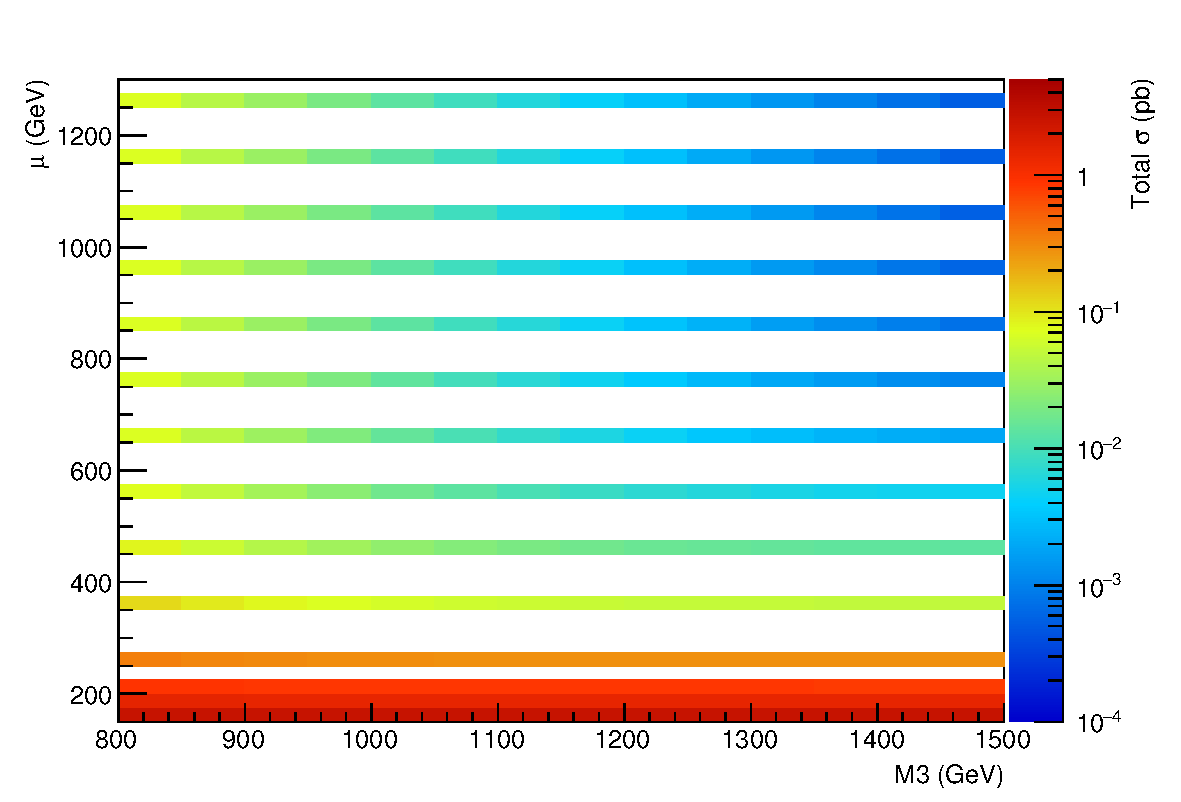
\includegraphics[width=0.49\textwidth]{figures/SigXsec_total}
%%   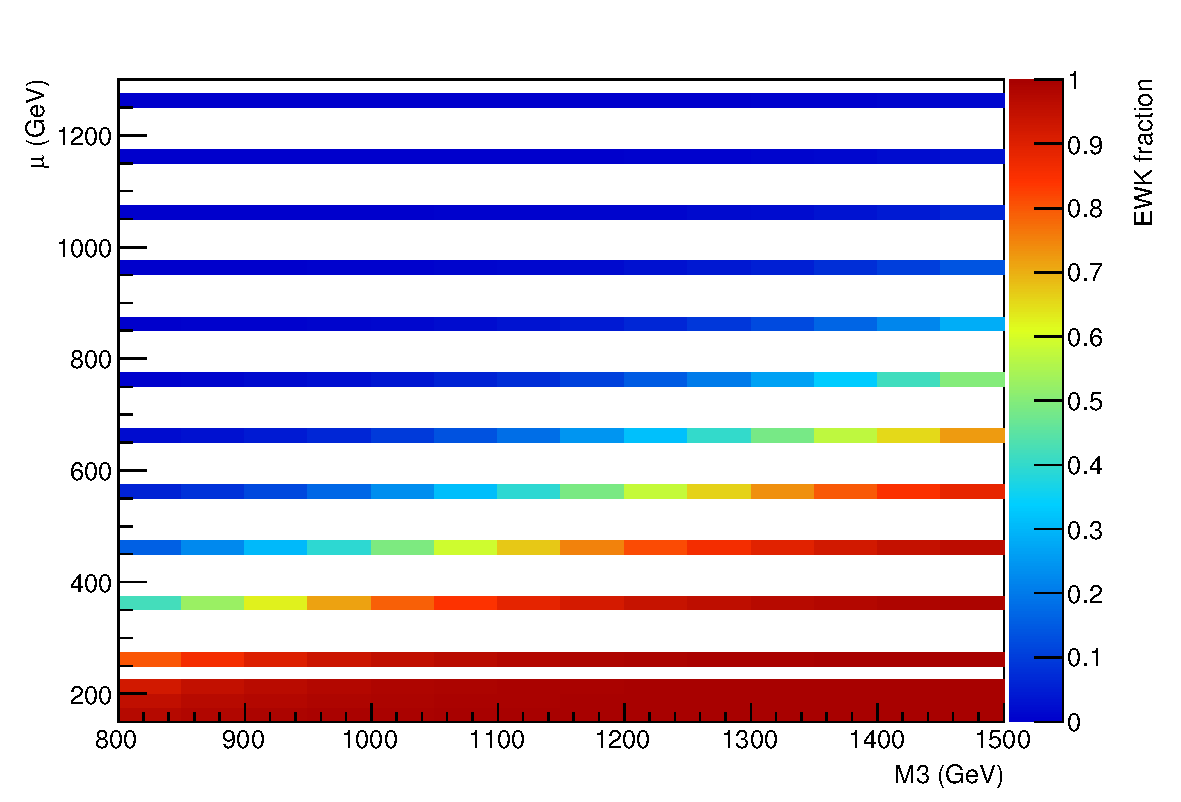
\includegraphics[width=0.49\textwidth]{figures/SigXsec_ewkFrac}
%%   \caption{Sección eficaz total (izquierda) y fracción relativa
%%     de producción EWK (derecha).}
%%   \label{fig:signal_xs_total}
%% \end{figure}

\section{Simulación de los fondos del SM}
\label{sec:bkg_samples}

%% Existen muchos procesos del {\SM} que pueden aparentar
%% una señal de SUSY con fotones, jets y energía faltante.
%% Estos pueden dividirse en varias categorías:

%% \begin{itemize}
%% \item {\MET} real (EWK)
%%   \begin{itemize}
%%   \item $\gamma$ real
%%     \begin{itemize}
%%     \item $Z(\to\nu\nu)+\gamma$
%%     \item $W(\to\tau\nu)+\gamma$, hadronic $\tau$-decay
%%     \item $W(\to e\nu)+\gamma$, the e is not reconstructed
%%     \item $W(\to\mu\nu)+\gamma$ and $W(\to\tau\nu)+\gamma$, the $\mu / \tau$ is not reconstructed
%%     \item $t\bar{t}+\gamma$,  the e$/ \mu$ (when produced) is not reconstructed
%%     \end{itemize}

%%   \item Electron$/$Jet faking photon
%%     \begin{itemize}
%%     \item $W(\to l\nu)$+jets
%%     \item $Z(\to \nu\nu)+$jets
%%     \item $t\bar{t}$
%%     \item dibosons
%%     \end{itemize}
%%   \end{itemize}

%% \item {\MET} instrumental
%%   \begin{itemize}
%%   \item $\gamma$ real ($\gamma+$jets)
%%   \item $\gamma$ falso (multijet, $Z(\to ll)+$jets)
%%   \end{itemize}
%% \end{itemize}

%% Las muestras simuladas con MC utilizadas en este analisis se describen
%% a continuacion. Como se discutira en la {\Sec} \ref{sec:background_estimation},
%% la contaminacion de fotones mal dentificados provenientes de jets y electrones
%% es estimado con metodos basados en datos. Sin embargo, las muestras MC tambien
%% han sido consideradas en estos casos para los estudios de optimizacion y la
%% evaluacion de las incertezas sistematicas.

%% \subsection{W/Z$+\gamma$}

%% Se espera que la produccion de {\wgam} y {\zgam} sea un fondo importante
%% para esta busqueda. Ambas muestras fueron generadas usando el generador
%% de eventos {\sherpa} v1.4.1 \cite{SherpaGen}, con hasta 3 partones en el
%% ME+PS y usando las funciones de densidad partonica CT10.
%% La combinacion de los elementos de matriz con las lluvias partonicas
%% es realizada de acuerdo a un procedimiento mejorado CKKW \cite{Catani:2001cc,Krauss:2002up}.
%% Un filtro a nivel generados es aplicado requiriendo al menos un foton
%% con $\pt > 80(70) \gev$ en el estado final de las muestras de {\wgam} (\zgam).
%% %option1
%% %Only leptonic decays of the Z were considered, including its invisible decay Z$\to\nu\nu$. Additional samples of \wgamma events with some variation of the simulation settings were used to compute systematic uncertainties on the expected yields for this background. All \Vgamma samples are listed in {\tab} \ref{tab:bkg_wzgamma_samples}.
%% %option2
%% Todos los decaimientos leptonicos del boson $Z$ fueron considerados,
%% incluyendo el decaimiento invisible $Z\to\nu\nu$.
%% Tambien se tuvo en cuenta un muestra de $V(\to qq)+\gamma  (V=W,Z/\gamma*)$
%% debido a que cierta energia faltante real puede  ser producida en el caso
%% de heavy flavour decays.
%% %Their contribution had been found negligible in all regions here considered. \tosolve{CHECK!}
%% %

%% \begin{table}[ht!]
%%   \centering
%%   \caption{Muestras de W/Z$+\gamma$ utilizadas en este analisis.
%%     La seccion eficas a LO se especifica para cada modo de decaimiento,
%%     al igual que los factores $k$, y las eficiencias del filtro.
%%     La luminosidad integrada correspondiente a la estadistica total
%%     de cada muestra esta tambien presente.}
%%   %\includegraphics[width=1\textwidth]{figures/tabla}
%%   \begin{tabular}{ l | c | c | c | c }
%%     \hline
%%     \hline
%%     Proceso (ID) & $\sigma~[pb]$ & $k$ & Eficiencia & $L [fb^{-1}]$ \\
%%     \hline
%%     {\wenugam} {\sherpa} (126741) &  0.7193  &  1.0  &  1.0  &  695.16 \\
%%     {\wmunugam} {\sherpa}  (126744) &  0.7178  &  1.0  &  1.0  &  696.56 \\
%%     {\wtaunugam} {\sherpa}  (158727) &  0.7199  &  1.0  &  1.0  &  694.57 \\
%%     {\zeegam} {\sherpa}  (158728) &  0.1861  &  1.0  &  1.0  &  1069.53 \\
%%     {\zmumugam} {\sherpa}  (158729) &  0.1858  &  1.0  &  1.0  &  1076.71 \\
%%     {\ztautaugam} {\sherpa}  (158730) &  0.1858  &  1.0  &  1.0  &  1076.19 \\
%%     {\znunugam} {\sherpa}  (126022) &  0.7625  &  1.0  &  1.0  &  655.74 \\
%%   %%   % in case we use this in the end 'option2'
%%     {\vqqgam} {\sherpa}  (164438) &  6.756  &  1.0  &  1.0  &  89.0 \\
%%   %%   \hline
%%   %%   \hline
%%   %%   \multicolumn{5}{l}{Systematics variations} \\
%%   %%   \hline
%%   %%    \wenugam (fact. 0.25x) \sherpa (204733) &  0.7193  &  1.0  &  1.0  &  278.05 \\
%%   %%    \wenugam (fact. 4x) \sherpa (204734) &  0.7193  &  1.0  &  1.0  &  278.05 \\
%%   %%    \wenugam (renorm. 0.25x) \sherpa (204735) &  0.7193  &  1.0  &  1.0  &  278.05 \\
%%   %%    \wenugam (renorm. 4x) \sherpa (204736) &  0.7193  &  1.0  &  1.0  &  278.05 \\
%%   %%    \wenugam (ckkw 15) \sherpa (204731) &  0.7193  &  1.0  &  1.0  &  278.05 \\
%%   %%    \wenugam (ckkw 30) \sherpa (204732) &  0.7193  &  1.0  &  1.0  &  278.05 \\
%%   %%    \wmunugam (fact. 0.25x) \sherpa (204739) &  0.7193  &  1.0  &  1.0  &  278.63 \\
%%   %%    \wmunugam (fact. 4x) \sherpa (204740) &  0.7193  &  1.0  &  1.0  &  278.63 \\
%%   %%    \wmunugam (renorm. 0.25x) \sherpa (204741) &  0.7193  &  1.0  &  1.0  &  278.63 \\
%%   %%    \wmunugam (renorm. 4x) \sherpa (204742) &  0.7193  &  1.0  &  1.0  &  278.63 \\
%%   %%    \wmunugam (ckkw 15) \sherpa (204737) &  0.7193  &  1.0  &  1.0  &  278.63 \\
%%   %%    \wmunugam (ckkw 30) \sherpa (204738) &  0.7193  &  1.0  &  1.0  &  278.63 \\
%%   %%    \wtaunugam (fact. 0.25x) \sherpa (204745) &  0.7193  &  1.0  &  1.0  &  277.81 \\
%%   %%    \wtaunugam (fact. 4x) \sherpa (204746) &  0.7193  &  1.0  &  1.0  &  277.81 \\
%%   %%    \wtaunugam (renorm. 0.25x) \sherpa (204747) &  0.7193  &  1.0  &  1.0  &  277.81 \\
%%   %%    \wtaunugam (renorm. 4x) \sherpa (204748) &  0.7193  &  1.0  &  1.0  &  277.81 \\
%%   %%    \wtaunugam (ckkw 15) \sherpa (204743) &  0.7193  &  1.0  &  1.0  &  277.81 \\
%%   %%    \wtaunugam (ckkw 30) \sherpa (204744) &  0.7193  &  1.0  &  1.0  &  277.81 \\
%%     \hline
%%     \hline
%%   \end{tabular}
%%   \label{tab:bkg_wzgamma_samples}
%% \end{table}

%% \subsubsection{W/Z+jets} \label{mc_wzjets}

%% Se espera que la produccion de W$^{\pm}$ y bosones $Z$ en asociacion con jets
%% contribuya a esta busqueda, con los fotones provenientes de electrones y jets
%% mal identificados. Especialemente para los segundos, esta contaminacion no esta
%% bien descripta por el MC. Por esta razon se utilizan metodos basados en datos
%% para estimar su contirbucion en las diferentes regiones de senal y control, como
%% se describe en el Capítulo \ref{cap:fondos}. De igual maner varias muestras de MC
%% fueron consideradas para validar los metodos.

%% Como se describe en el Capítulo \ref{cap:seleccion} la seleccion de senal involucra
%% muchos jets en el estado final, es importante modelar los estados final multipartonicos
%% de forma adecuada. Con esto en mente, el generador de events {alpgen} (version 2.14)
%% fue utilizado, incluyendo los efectos EWK y QCD a LO para los procesos de interaccion
%% fuerte multipartonicos. La produccion de jets fue generada for up to five-parton
%% matrix elements. Este generados fue interfaceado con {\herwig} version 6.5.2
%% para la simulacion de las lluvias y los procesos de fragmentacion y con {\jimmy}
%% para la simulacion de los eventos subyacentes. Las funciones de densidad partonica
%% utilizadas fueron las CTEQ6L1. La normalizacion a la luminosidad integrada acumulada
%% fue hecha escalenado la seccion eficas mostrada en la {\tab} \ref{tab:bkg_wzjets_samples}
%% usando calculos QCD a NNLO de el programa FEWZ \cite{Anastasiou:2003ds}.
%% En cada caso los mismos factores de normalizacion fueron aplicados a los elementos
%% de matriz de {\alpgen}.
%% %%applied for all \alpgen matrix element parton multiplicities.
%% Finalmente, se realiza la remocion de eventos para evitar el conteo doble de eventos
%% que ya fueron tenidos en cuenta por las muestras de Z$\gamma$ y W$\gamma$.
%% Para esto, los eventos de $W(Z)+\text{jets}$ con fotones con $\pt > 80(70)\gev$
%% y $\Delta{\rm R}(e/\mu/\tau/$light-quarks$, \gamma) > 0.1$ fueron removidos
%% de las muestras.

\begin{table}[ht!]
  \centering
  \caption{Muestras de $W/Z+\text{jets}$ utilizadas en este analisis. {\mccaption}.}
  \begin{tabular}{lcccc}
    \hline
    \hline
    Proceso & $\sigma [pb]$ & factor-$k$ & Eficiencia & $L [fb^{-1}]$ \\
    \hline
    \zeenj{0}  \alpgen+\jimmy  & 711.77 & 1.23 & 1 & 7.548 \\
    \zeenj{1}  \alpgen+\jimmy  & 155.17 & 1.23 & 1 & 6.994 \\
    \zeenj{2}  \alpgen+\jimmy  & 48.745 & 1.23 & 1 & 6.746 \\
    \zeenj{3}  \alpgen+\jimmy  & 14.225 & 1.23 & 1 & 6.286 \\
    \zeenj{4}  \alpgen+\jimmy  & 3.7595 & 1.23 & 1 & 6.487 \\
    \zeenj{5}  \alpgen+\jimmy  & 1.0945 & 1.23 & 1 & 7.428 \\
    \zmmnj{0}  \alpgen+\jimmy  & 712.11 & 1.23 & 1 & 7.557 \\
    \zmmnj{1}  \alpgen+\jimmy  & 154.77 & 1.23 & 1 & 7.011 \\
    \zmmnj{2}  \alpgen+\jimmy  & 48.912 & 1.23 & 1 & 6.731 \\
    \zmmnj{3}  \alpgen+\jimmy  & 14.226 & 1.23 & 1 & 6.286 \\
    \zmmnj{4}  \alpgen+\jimmy  & 3.7838 & 1.23 & 1 & 6.445 \\
    \zmmnj{5}  \alpgen+\jimmy  & 1.1148 & 1.23 & 1 & 7.292 \\
    \zttnj{0} \alpgen+\jimmy  & 711.81 & 1.23 & 1 &  7.560 \\
    \zttnj{1} \alpgen+\jimmy  & 155.13 & 1.23 & 1 &  6.996 \\
    \zttnj{2} \alpgen+\jimmy  & 48.804 & 1.23 & 1 &  6.746 \\
    \zttnj{3} \alpgen+\jimmy  & 14.160 & 1.23 & 1 &  6.315 \\
    \zttnj{4} \alpgen+\jimmy  & 3.7744 & 1.23 & 1 &  6.462 \\
    \zttnj{5} \alpgen+\jimmy  & 1.1163 & 1.23 & 1 &  7.283 \\
    \hline
    \wenunj{0}  \alpgen+\jimmy  &8037.10   & 1.186 & 1 & 0.362 \\
    \wenunj{1}  \alpgen+\jimmy  &1579.20   & 1.186 & 1 & 1.334 \\
    \wenunj{2}  \alpgen+\jimmy  &477.20     & 1.186 & 1 & 6.661 \\
    \wenunj{3}  \alpgen+\jimmy  &133.93     & 1.186 & 1 & 6.358 \\
    \wenunj{4}  \alpgen+\jimmy  &35.62       & 1.186 & 1 &  5.917\\
    \wenunj{5}  \alpgen+\jimmy  &10.55       & 1.186 & 1 &  5.592\\
    \wmnunj{0}  \alpgen+\jimmy  &8040.00 & 1.186 & 1 &  0.363\\
    \wmnunj{1}  \alpgen+\jimmy  &1580.30 & 1.186 & 1 &  1.333\\
    \wmnunj{2}  \alpgen+\jimmy  &477.50   & 1.186 & 1 &  6.656\\
    \wmnunj{3}  \alpgen+\jimmy  &133.94   & 1.186 & 1 &  6.357\\
    \wmnunj{4}  \alpgen+\jimmy  &35.64      & 1.186 & 1 &  6.033\\
    \wmnunj{5}  \alpgen+\jimmy  &10.57      & 1.186 & 1 &  1.595\\
    \wtnunj{0} \alpgen+\jimmy     &8035.80  & 1.186 & 1 & 0.353 \\
    \wtnunj{1} \alpgen+\jimmy     &1579.80  & 1.186 & 1 & 1.307 \\
    \wtnunj{2} \alpgen+\jimmy     &477.55    & 1.186 & 1 &  6.567\\
    \wtnunj{3} \alpgen+\jimmy     &133.79    & 1.186 & 1 &  6.365\\
    \wtnunj{4} \alpgen+\jimmy     &35.58      & 1.186 & 1 &  5.921\\
    \wtnunj{5} \alpgen+\jimmy     &10.54      & 1.186 & 1 &  5.199\\
    \hline
    \hline
  \end{tabular}
  \label{tab:bkg_wzjets_samples}
\end{table}


\subsubsection{Top pair ($+\gam$) production}\label{sec:mcttbargam}

Otro fondo importante para este analisis es el {\ttgam}. Esta muestra MC fue generada
utilizando {\madgraph}\cite{Alwall:2007st} y la PDF CTEQ6L1.
{\pythiasix}\cite{pythia} fue usado para la simulacion de las lluvias partonicas, fragmentación y
eventos subyacentes. La radiacion de fotones fue agregadas utilizando
{\photos}\cite{photos}, y los decaimientos de los leptones tau con
{\tauola} \cite{tauola}.
Se requirio que los fotones a nivel generador tengan un
$\pt > 80 \gev$.
Para evitar efectos cinematicos introducidos por el filtro, el corte en el {\pt}
del foton en la muestra reconstruida se aumento a 95 {\gev}.
Se utilizo un factor-$k$ de $1.9 \pm 0.4$\cite{Melnikov:2011ta, tth}. %This was calculated by
%% %the theorists with the particular generator-level cuts used to                                                                                                                     %generate this MC sample.

Los detalles de la simulacion se encuentran en la \cref{tab:bkg_ttbar_samples}.
Se utilizaron ademas algunas muestras a nivela general como variaciones para calculas
las incertezas sistematicas como se explica en la \cref{sec:syst_ttbargamma}.


%% % NOT ANYMORE , but explained later why
%% %As described in {\sec} \ref{}, the normalization of this sample was extracted together with that for %W$+\gamma$ events by fitting
%% %simultaneously the two MC to data in specifically designed control regions.

%% %More information can be found in
%% %Ref.~\cite{ttbargammaSupport}.

La produccion de {\ttbar}, donde los electrones o los jets
son mal identificados como fotones es una fuente de fondo que
vale la pena considerar.
Aunque ambas contaminacions fueron estimadas a partir de los datos, eventos simulados fueron
utilizados en la etapa de optimizacion y para chequeos de los metodos DD. La
muestra MC fue generada utilizando {\powheg}\cite{Nason:2004rx,Frixione:2007vw,Alioli:2010xd}
con la lluvia partonica y fragmentacion hecha por {\pythia}.
Para el UE se utilizo Perugia 2011C \footnote{see some details at \url{https://twiki.cern.ch/twiki/bin/viewauth/AtlasProtected/P2011C}.}
con el conjunto de PDFs CTEQ6L1 LO.
La radiacion de fotones adicional fue agregada con {\photos} \cite{photos}.
Overlap removal is performed to prevent double-counting the phase-space
covered by the {\ttgam} MC sample. Events with truth prompt photons with
$\pt > 95 \gev$ and $\Delta{\rm R}(e/\mu/\tau/g/$light-quarks$, \gamma) > 0.1$ are removed from the \ttbar\ sample.


\begin{table}[ht!]
  \centering
  \caption{{\ttgam} samples used for the analysis. {\mccaption}}

  \begin{tabular}{lcccc}
    \hline
    \hline
    Proceso & $\sigma [pb]$ & factor-$k$ & Eficiencia & $L [fb^{-1}]$ \\
    \hline
    \hline
    \ttbar\ \powheg+\pythia & 253.00 & 1 & 0.543 & 580 \\
    \hline
    %    \ttbargam noAllHad \madgraph (164439) & 0.092363 & 1.9 & 1 & 1139.7 \\
    {\ttgam} noAllHad \madgraph & 0.09873 & 1.9 & 1 & 1066.2 \\
    {\ttgam} AllHad \madgraph  & 0.068599 & 1.9 & 1 & 1534.5 \\
    \hline
    \hline
    \multicolumn{5}{l}{Variaciones sistematicas} \\
    \hline
    {\ttgam} noAllHad (scaleUP) \madgraph & 0.09873 & 1.9 & 1 & 1066.2 \\
    {\ttgam} noAllHad (scaleDN) \madgraph & 0.09873 & 1.9 & 1 & 1066.2 \\
    {\ttgam} noAllHad (alpsUP)  \madgraph & 0.09873 & 1.9 & 1 & 1066.2 \\
    {\ttgam} noAllHad (alpsDN)  \madgraph & 0.09873 & 1.9 & 1 & 1066.2 \\
    {\ttgam} noAllHad (moreFSR) \madgraph & 0.09873 & 1.9 & 1 & 1066.2 \\
    {\ttgam} noAllHad (lessFSR) \madgraph & 0.09873 & 1.9 & 1 & 1066.2 \\
    \hline
    \hline
  \end{tabular}
  \label{tab:bkg_ttbar_samples}
\end{table}

\subsubsection{Single top (+ $\gamma$)}

Single top con un foton asociado fue generado utilizando
Whizard 2.1.1 \cite{whizard, whizard2}, con 4-flavor/5-flavor
matching provided using Hoppet~\cite{hoppet}.\footnote{Thanks to
  abian Bach for providing an early version of the matching, which
  will be standard in Whizard 2.2.0.}
El foton extra photon could be in
%% either the single top production or the subsequent decays. Production
%% and decay, however, was treated separately, so interference effects
%% are ignored. {\pythia} \cite{pythia} was used for parton showering and
%% fragmentation. Additional photon radiation was added with
%% {\photos} \cite{photos}, and tau leptons were decayed with
%% {\tauola} \cite{tauola}.

%% %We used sample IDs 202621 and 202622 for \tchangamma production, and
%% %sample IDs 202623--202631 for \tWgamma production.

\begin{table}[ht!]
  \centering
  \caption{Single top and \tgam\ samples used for the analysis. La seccion eficas a
    NNLO, eficiencia del filtro, y luminosidad integrada correspondiente a la estadística total de cada muestra
    se detallan.}
  \begin{tabular}{lccc}
    \hline
    Proceso & $\sigma [pb]$ & Eficiencia & $L [fb^{-1}]$ \\
    \hline
    t-channel \acermc   & 28.4 & 1 & 271 \\
    Wt        \powheg   & 22.4 & 1 & 892 \\
    s-channel \powheg   & 1.82 & 1 & 3299 \\
    \hline
    \tgam (t-channel) \wizhard+\pythia   & 0.187298 & 0.121980 & 4810 \\
    \tgam (t-channel) \wizhard+\pythia   & 0.313866 & 0.012927 & 4930 \\
    \hline
    \twgam (dilep.) \wizhard+\pythia          & 0.01292  & 0.16437 & 4710 \\
    \twgam (dilep. tDec) \wizhard+\pythia     & 0.01454  & 0.02875 & 12000 \\
    \twgam (dilep. WDec) \wizhard+\pythia     & 0.01041  & 0.07549 & 6370 \\
    \twgam (tlepWhad) \wizhard+\pythia        & 0.02583  & 0.16244 & 4770 \\
    \twgam (tlepWhad tDec) \wizhard+\pythia   & 0.02908  & 0.02761 & 6230 \\
    \twgam (tlepWhad WDec) \wizhard+\pythia   & 0.01159  & 0.06471 & 6660 \\
    \twgam (thadWlep) \wizhard+\pythia )      & 0.02582  & 0.16178 & 4790 \\
    \twgam (thadWlep tDec) \wizhard+\pythia   & 0.02013  & 0.04198 & 5920 \\
    \twgam (thadWlep WDec) \wizhard+\pythia   & 0.02079  & 0.07574 & 3180 \\
    \hline
    \hline
  \end{tabular}
  \label{tab:bkg_st_samples}
\end{table}

%% The single top process is a small background for this analysis, mostly
%% important for the control and validation regions. $Wt$ production (ID 110140) was generated using the \powheg, including full next-to-leading order QCD
%% corrections. Parton showering and fragmentation were simulated by
%% \pythia with the P2011C tune. The CT10 next-to-leading-order parton
%% set is used for the matrix element, the parton shower and the
%% underlying event. The samples were scaled to the cross section
%% calculated in \cite{Kidonakis:2010ux}. For $t$-channel
%% production, the MC samples with sample ID 110101 were used, with the
%% $W$ boson decaying leptonically. These were generated with
%% \acermc \cite{acer}, with parton showering and fragmentation performed
%% by {\pythia} with the P2011C tune and CTEQ6L1 PDF set.  The samples were
%% scaled to the cross section calculated by \cite{Kidonakis:2011wy}.
%% Single top produced by $s$-channel was not used because it was found
%% to be negligible.

%% Overlap between the single top and single top $\gamma$ samples has been removed.

\subsubsection{Direct $\gamma+$jets and QCD multijet}

%% %The QCD background is one of the main source of background in this analysis, particularly prompt photon events. The QCD contamination is in all cases a result of pathological events (jet faking a photon, badly reconstructed jet or photon making high \MET) for which the simulation is not reliable.
%% %For this reason this background is computed with a data driven approach, as explained in {\sec} \ref{sec:jetsmearing}. Several MC simulations are used anyways for consistency checks and to assess systematic uncertainties.

%% The QCD contamination is in all cases a result of pathological events
%% (jet faking a photon, badly reconstructed jet or photon making high \MET).
%% However, it is not expected to be a dominant source of background in the
%% phase space explored in this analysis. The contribution from events with
%% jets faking a photon is estimated with the data driven described in
%% {\Sec} \ref{sec:jetfakes}. The QCD multijet samples listed in {\tab}
%% \ref{tab:bkg_qcd_samples} were used for optimisation and preliminar
%% sensitivity studies. Prompt photon production was simulated with
%% with {\sherpa} v1.4.1 \cite{SherpaGen}, with up to four partons in the ME+PS
%% and using the CT10 set of parton density functions. The inclusive spectrum
%% is sliced in ranges of photon \pt\ to optimise the event generation.
%% Alternative samples were used to asses systematics uncertainties and
%% cross checks, generated with {\pythiaeight} (using CTEQ6L1) and {\alpgen}
%% v2.14 (with same config as V$+$jets events described in {\Sec} \ref{mc_wzjets}).
%% Further details are given in {\tab} \ref{tab:bkg_qcd_samples}.

\begin{table}[ht!]
  \centering
  \caption{Muestras de QCD {\gjet} y multijet utilizadas en este analisis.
    La seccion eficas a LO para cada modo de decaimiento,
    y las eficiencias del filtro son reportadas,
    asi como tabine la luminosidad integrada correspondiente a la estadistica
    total de cada muestra.}

  %% \includegraphics[width=1\textwidth]{figures/tabla}

   \begin{tabular}{lccc}
    \hline
    \hline
    Proceso & $\sigma [pb]$ & Eficiencia & $L [fb^{-1}]$ \\
    \hline
    {\gjet} ($\pt>70\gev$)   &   2153.0  &  1.0  &  1.160 \\
    {\gjet} ($\pt>140\gev$)  &   137.85  &  1.0  &  10.881 \\
    {\gjet} ($\pt>280\gev$)  &    5.963  &  1.0  &  167.657 \\
    {\gjet} ($\pt>500\gev$)  &    0.276  &  1.0  &  3617.291 \\
    {\gjet} ($\pt>800\gev$)  &   0.0133  &  1.0  &  7492.807 \\
    {\gjet} ($\pt>1000\gev$) &  0.00238  &  1.0  &  41980.269 \\
    \hline
    {\gjet} ($\pt>70\gev$)   &  3425000  &  $5.7 \times 10^{-4}$  &  1535.4  \\
    {\gjet} ($\pt>140\gev$)  &   122170  &  $9.7 \times 10^{-4}$  &  8449.2 \\
    {\gjet} ($\pt>280\gev$)  &   3348.7  &  $1.45 \times 10^{-3}$ &  206559.7 \\
    {\gjet} ($\pt>500\gev$)  &   115.63  &  $1.8 \times 10^{-3}$  &  4789097.0\\
    \hline

    \gjetnj{1} ($\pt>70\gev$)   &  577.480  &  1.0  &  0.147 \\
    \gjetnj{1} ($\pt>140\gev$)  &  26.198   &  1.0  &  3.626 \\
    \gjetnj{1} ($\pt>280\gev$)  &  0.83119  &  1.0  &  30.077 \\
    \gjetnj{1} ($\pt>500\gev$)  &  0.02914  &  1.0  &  343.159 \\

    % \gjetnj{2} ($\ptgam>35\gev$) \alpgen+\jimmy  ( 156846 ) &  4515.0  &  1.0  &  0.00886 \\
    \gjetnj{2} ($\pt>70\gev$)    &  571.870  &  1.0  &  0.175 \\
    \gjetnj{2} ($\pt>140\gev$)   &  38.67100  &  1.0  &  3.879 \\
    \gjetnj{2} ($\pt>280\gev$)   &  1.6811  &  1.0  &  29.741 \\
    \gjetnj{2} ($\pt>500\gev$)   &  0.075517  &  1.0  &  264.841 \\

    % \gjetnj{3} ($\ptgam>35\gev$) \alpgen+\jimmy  ( 156851 ) &  1717.0  &  1.0  &  0.00874 \\
    \gjetnj{3} ($\pt>70\gev$)  &  306.10  &  1.0  &  0.049\\
    \gjetnj{3} ($\pt>140\gev$) &  28.57  &  1.0  &  5.250 \\
    \gjetnj{3} ($\pt>280\gev$) &  1.538  &  1.0  &  32.503 \\
    \gjetnj{3} ($\pt>500\gev$) &  0.07707  &  1.0  &  77.822 \\

    % \gjetnj{4} ($\ptgam>35\gev$) \alpgen+\jimmy  ( 156856 ) &  513.940002  &  1.0  &  0.00778 \\
    \gjetnj{4} ($\pt>70\gev$)    &  115.850  &  1.0  &  0.216 \\
    \gjetnj{4} ($\pt>140\gev$)   &  14.216  &  1.0  &  11.951 \\
    \gjetnj{4} ($\pt>280\gev$)   &  0.9185  &  1.0  &  48.992 \\
    \gjetnj{4} ($\pt>500\gev$)   &  0.0512  &  1.0  &  156.354 \\

    % \gjetnj{5} ($\ptgam>35\gev$) \alpgen+\jimmy  ( 156861 ) &  163.800003  &  1.0  &  0.0458 \\
    \gjetnj{5} ($\pt>70\gev$)    &  7.00  &  1.0  &  18.569 \\
    \gjetnj{5} ($\pt>140\gev$)   &  0.542  &  1.0  &  92.304 \\
    \gjetnj{5} ($\pt>280\gev$)   &  0.0333  &  1.0  &  450.911 \\
    \gjetnj{5} ($\pt>500\gev$)   &  44.334  &  1.0  &  0.970 \\
    \hline
    \hline
    JZ1W ($20 \gev < \pt^{\mathrm{jet}} < 80 \gev$)      &  $7.285 \times 10^{10}$ &  0.000129 & 0.00016 \\
    JZ2W ($80 \gev < \pt^{\mathrm{jet}} < 200 \gev$)     &  $2.634 \times 10^{7}$ &  0.003894 & 0.0142 \\
    JZ3W ($200 \gev < \pt^{\mathrm{jet}} < 500 \gev$)    &  $5.442 \times 10^{5}$ &  0.001219 & 2.26 \\
    JZ4W ($500 \gev < \pt^{\mathrm{jet}} < 1000 \gev$)   &  $6.445 \times 10^{3}$ &  0.000708 & 328 \\
    JZ5W ($1000 \gev < \pt^{\mathrm{jet}} < 1500 \gev$)  &  39.74 &  0.002152 & 17400 \\
    JZ6W ($1500 \gev < \pt^{\mathrm{jet}} < 2000 \gev$)  &  0.4161 &  0.004684 & $7.68 \times 10^{5}$ \\
    JZ7W ($\pt^{\mathrm{jet}} > 2000 \gev$)              &  0.04064 &  0.0146 & $2.52\times 10^{6}$ \\
    \hline
  \end{tabular}
  \label{tab:bkg_qcd_samples}
\end{table}

\subsubsection{Dibosons}

Los procesos de diboson (WW, WZ, y ZZ) fueron generados utilizando
{\sherpa} y usando la PDF CT10, con la seccion eficaz provista por
MCFM \cite{Campbell:2011bn}. Solo los decaimientos leptonicos para
ambos bosones fueron considerados.

\begin{table}[ht!]
  \centering
  \caption{Muestras de Diboson utilizadas en este análisis.
    La sección eficaz a LO para cada modo de decaimiento, los factores $k$
    (para la normalización NLO) y las eficiencias del filtro están detalladas,
    así como también la luminosidad integrada correspondiente a la estadística
    total de cada muestra.}

  \begin{tabular}{lcccc}
    \hline
    Proceso & $\sigma [pb]$ & factor $k$ & Eficiencia & $L [fb^{-1}]$ \\
    \hline
    %% $WW(2l2\nu)$ \sherpa (126892)  & 5.50 & 1.07 & 1 & 458.9 \\
    %% $WZ(3l)$ \sherpa (126893) & 9.75 & 1.06 & 1 & 261.1 \\
    %% $ZZ(4\ell)$ \sherpa (126894)  & 8.74 & 1.11 & 1  &  185.6 \\
    %% $ZZ(2\ell2\nu)$ \sherpa (126895)  & 0.50 & 1.14 & 1 &  1590.8 \\
    $WW (\ell\ell\nu\nu)$        & 5.296  & 1.06 & 1 & 1400 \\
    $ZZ (\ell\ell\nu\nu)$        & 0.494  & 1.05 & 1 & 1700 \\
    $WZ (\ell\ell\ell\nu)$       & 9.745  & 1.05 & 1 & 260 \\
    $WZ (\ell\nu\nu\nu)$         & 1.406  & 1.05 & 1 & 270 \\
    $ZW (eeqq)$                  & 1.465  & 1.05 & 1 & 110 \\
    $ZZ (eeqq)$                  & 0.247  & 1    & 1 & 120 \\
    $ZW (\mu\mu qq)$             & 1.463  & 1.05 & 1 & 110 \\
    $ZZ (\mu\mu qq)$             & 0.248  & 1    & 1 & 120 \\
    $ZW (\tau\tau qq)$           & 1.452  & 1.05 & 1 & 120 \\
    $ZZ (\tau\tau qq)$           & 0.242  & 1    & 1 & 120 \\
    $ZW (\nu\nu qq)$             & 2.697  & 1.05 & 1 & 64 \\
    $ZZ (\nu\nu qq)$             & 1.744  & 1    & 1 & 69 \\
    $WW (e\nu qq)$               & 7.285  & 1.06 & 1 & 100 \\
    $WZ (e\nu qq)$               & 1.904  & 1.05 & 1 & 110 \\
    $WW (\mu\nu qq)$             & 7.297  & 1.06 & 1 & 100 \\
    $WZ (\mu\nu qq)$             & 1.906  & 1.05 & 1 & 100 \\
    $WW (\tau\nu qq)$            & 7.274  & 1.06 & 1 & 100 \\
    $WZ (\tau\nu qq)$            & 1.915  & 1.05 & 1 & 100 \\
    \hline
  \end{tabular}
  \label{tab:bkg_diboson_samples}
 \end{table}



Referencias

%% MC Event Generators
@inproceedings{Seymour:2013ega,
  author         = ``Seymour, Michael H. and Marx, Marilyn'',
  title          = ``{Monte Carlo Event Generators}'',
  booktitle      = ``{Proceedings, 69th Scottish Universities Summer School in
    Physics : LHC Phenomenology (SUSSP69)}'',
  url            = ``http://inspirehep.net/record/1229804/files/arXiv:1304.6677.pdf'',
  year           = ``2013'',
  pages          = ``287-319'',
  doi            = ``10.1007/978-3-319-05362-2_8'',
  eprint         = ``1304.6677'',
  archivePrefix  = ``arXiv'',
  primaryClass   = ``hep-ph'',
  reportNumber   = ``MCNET-13-05'',
  SLACcitation   = ``%%CITATION = ARXIV:1304.6677;%%''
}

%% ATLAS Simulation
@article{
  year={2010},
  issn={1434-6044},
  journal={The European Physical Journal C},
  volume={70},
  number={3},
  doi={10.1140/epjc/s10052-010-1429-9},
  title={The ATLAS Simulation Infrastructure},
  url={http://dx.doi.org/10.1140/epjc/s10052-010-1429-9},
  publisher={Springer-Verlag},
  author={ATLAS Collaboration},
  pages={823-874},
  }

%% XS
@article{Kramer:2012bx,
  author         = ``Kramer, Michael and Kulesza, Anna and van der Leeuw,
  Robin and Mangano, Michelangelo and Padhi, Sanjay and
  Plehn, Tilman and Portell, Xavier'',
  title          = ``{Supersymmetry production cross sections in $pp$
    collisions at $\sqrt{s}=7$ TeV}'',
  year           = ``2012'',
  eprint         = ``1206.2892'',
  archivePrefix  = ``arXiv'',
  primaryClass   = ``hep-ph'',
  reportNumber   = ``CERN-PH-TH-2012-163'',
  SLACcitation   = ``%%CITATION = ARXIV:1206.2892;%%''
  }
